\section{Experiments and Results}
For all the plots of the experiments the red curve indicates the tumour cell density, the blue curve the ECM density and the green curve the MDE concentration. 
\subsection{Two dimensional Results}
\subsubsection{Replicating results}

%naming convention of figures: d0_d1_d2_eta_alpha_beta_gamma_mu1_mu2

\begin{figure}[h]
    \centering
    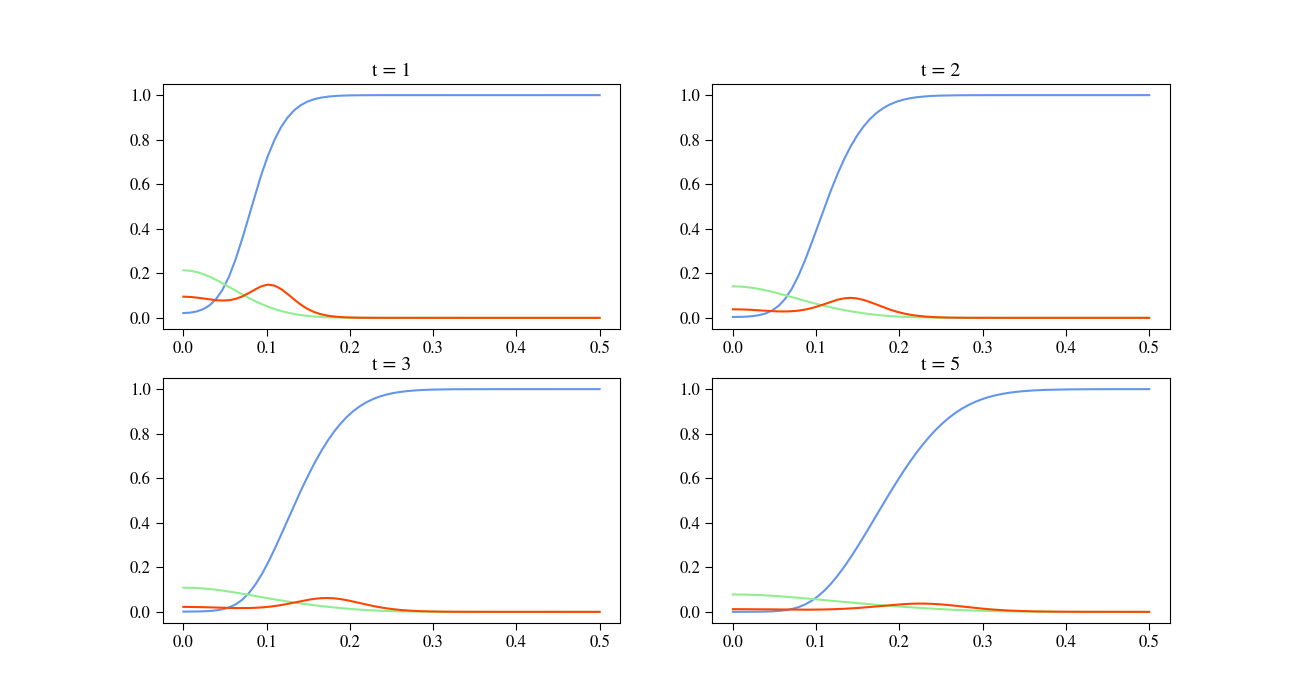
\includegraphics[width=\textwidth]{resources/images/0.001_0.001_0.001_10_0.1_0_0.005_0_0.png}
    \caption{Caption}
    \label{fig:0.001_0.001_0.001_10_0.1_0_0.005_0_0}
\end{figure}
In the first simulation the parameter values were used as follows $d_c = 0.001, d_m = 0.001, \gamma = 0.005, \eta = 10, \alpha = 10, \beta = 0, \mu_1 = 0, \mu_2 = 0$. Figure \ref{fig:0.001_0.001_0.001_10_0.1_0_0.005_0_0} shows 6 snapshots of different points in time of tumour cell density, extracellular matrix density and matrix degrading enzymes concentration. Starting from the inital values of figure (place correct refrence here) we see that a small cluster has formed at the leading edge of the tumour cells, this is due to the haptotactic flux having a higher value of 0.005 instead of 0.001 for random motility. This pulls the tumour cells towards the direction where the ECM is highest, into direction of the gradient of $e$. With passing time this cluster migrates furhter from the main body of the tumour outwards into the surrounding tissue, this happens when considering the points of time at a decreasing rate, where up unitl $t = 5$ the cluster has flatten, yet it is clearly visible. This cluster breaking away from the main body indicates the ability of the tumour cells to migrate and invade the adjacent area, starting the metastatic cascade, forming secondary tumour sites. 

% wrong parameters change later
\begin{figure}
    \centering
    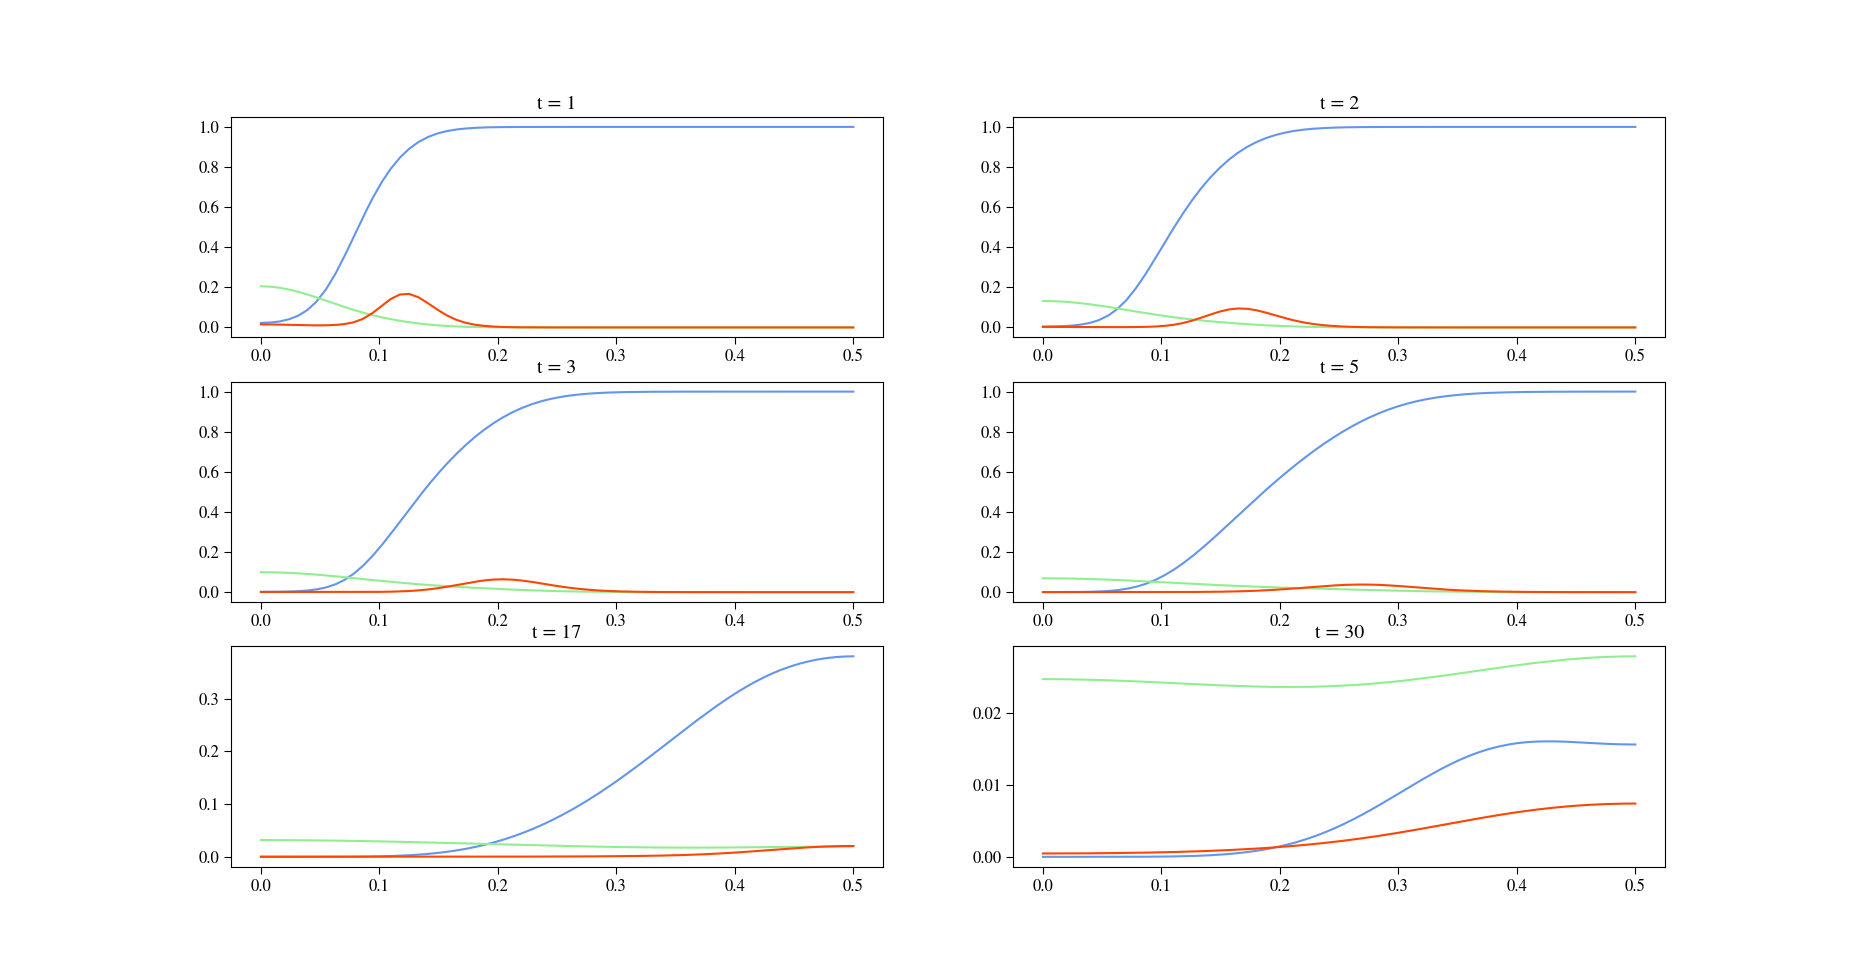
\includegraphics[width=\textwidth]{resources/images/0.001_0.001_0.001_10_0.1_0_0.01_0_0.png}
    \caption{Caption}
    \label{fig:0.001_0.001_0.001_10_0.1_0_0.01_0_0}
\end{figure}

The second experiments, figure \ref{fig:0.001_0.001_0.001_10_0.1_0_0.01_0_0}, has an increased value of $\gamma = 0.01$ and is for the remaing values similiar to experiment 1. Because of the larger haptotatic flux $\gamma$ the cluster at the leading edge of the tumour cells density is noticably higher than in the first experiment, the cells migrating faster into the tissue. This results in an also faster decay of the ECM density. In the last image at $t = 30$ we can clearly see that for $gamma = 0.01$ the MDE curve is considerably higher than both ECM density and the MDE concentration curve of experiment 1. 

\begin{figure}
    \centering
    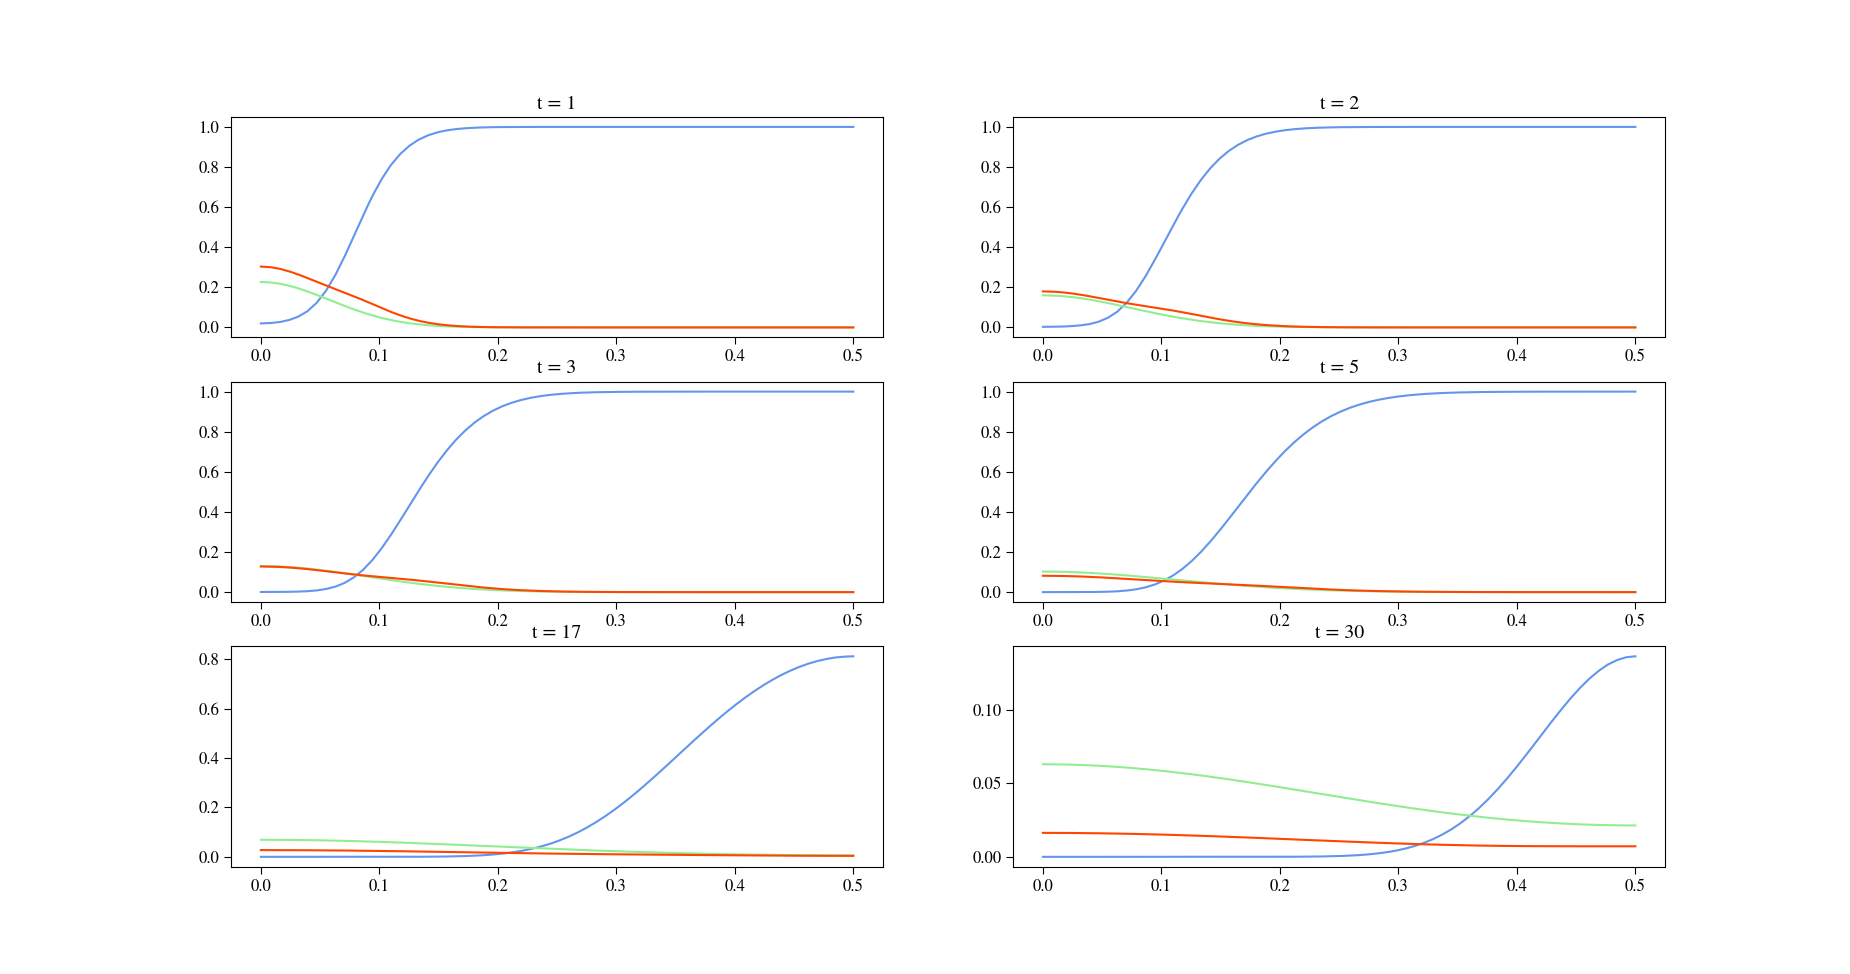
\includegraphics[width=\textwidth]{resources/images/0.001_0.001_0.001_10_0.1_0_0.001_0_0.png}
    \caption{Caption}
    \label{fig:0.001_0.001_0.001_10_0.1_0_0.001_0_0}
\end{figure}

Figure \ref{fig:0.001_0.001_0.001_10_0.1_0_0.001_0_0} shows the results of a simulation where $\gamma = 0.001$ is decreased and has similiar values for the other parameters as experiments 1,2. The cluster invading the tissue is almost not visible anymore and the migration process of the tumour cells happens, as was expected, slower than in the previous experiments. In the last image of this experiment at $t = 30$ we can see that if we compare it to the previous two experiments that ECM density is still higher than the MDE concentration, with the MDEs not having degraded the ECM structure this far outward from the origin. \newline
Drawing a first conclusion for the parameter of $\gamma$ we can observe that depending on it, as the name haptotactic flux coefficient also implies, the pace of the invasion of the surrounding tissue cruically depends on this and with this also the degradation of the moving farther away from the origin. This parameter also determines the scale of how well the tumour cells can invade the surrounding tissue, if this value low we see that there is almost no cluster leading at the edge, if the values is higher the cluster is more distinct which increases the ability to start the metastatic cascade.\newline
\begin{figure}
    \centering
    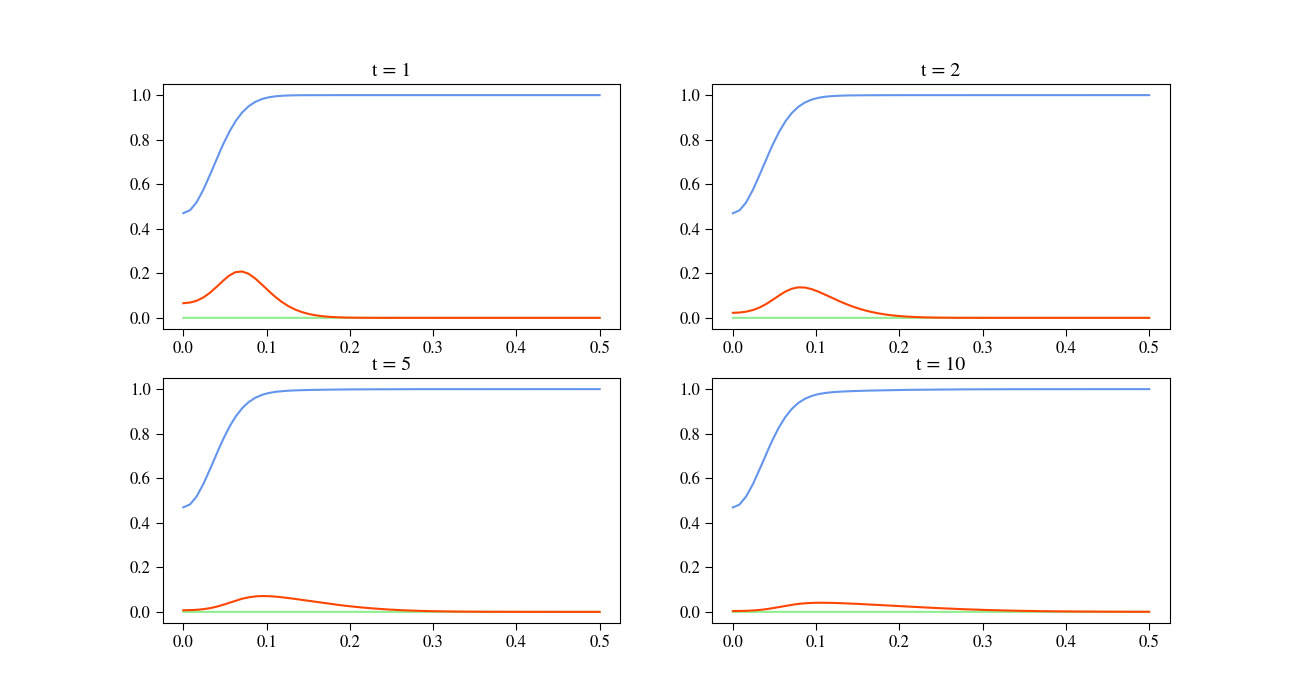
\includegraphics[width=\textwidth]{resources/images/0.001_0.001_0.001_10_0.1_0.5_0.005_0_0.png}
    \caption{Caption}
    \label{fig:0.001_0.001_0.001_10_0.1_0.5_0.005_0_0}
\end{figure}
In the next experiment, depicted in figure \ref{fig:0.001_0.001_0.001_10_0.1_0.5_0.005_0_0} the parameter $\beta = 0.5$ is changed leaving the rest the same. This introduces a decay term in the MDE concentration. Here we can also see the cluster forming at the edge, and also propagating towards the gradient of the ECM, but in contrast to the first experiment we see that the ECM is not temporaily degraded, being stable over time. Also the MDE concentration stays constant. These two observations of MDE concentration and ECM density suggest that the MDE decay term and the production term for MDEs coming from the tumourous cells stays in balance, over time both curves dont seem change dramatically, having the same final configuration as the initail condition. The movement of the tumour cells looks generally the same with the difference to the first experiment that the pace at which the cells migrate outwards into the surrounding area is slower, this only makes sense, since the ECM is constant and therefore the gradient term of it nullifies itself. With time the tumour cells migrate to the outer limit of the unit square and take on a constant distribution across space. 
\begin{figure}
    \centering
    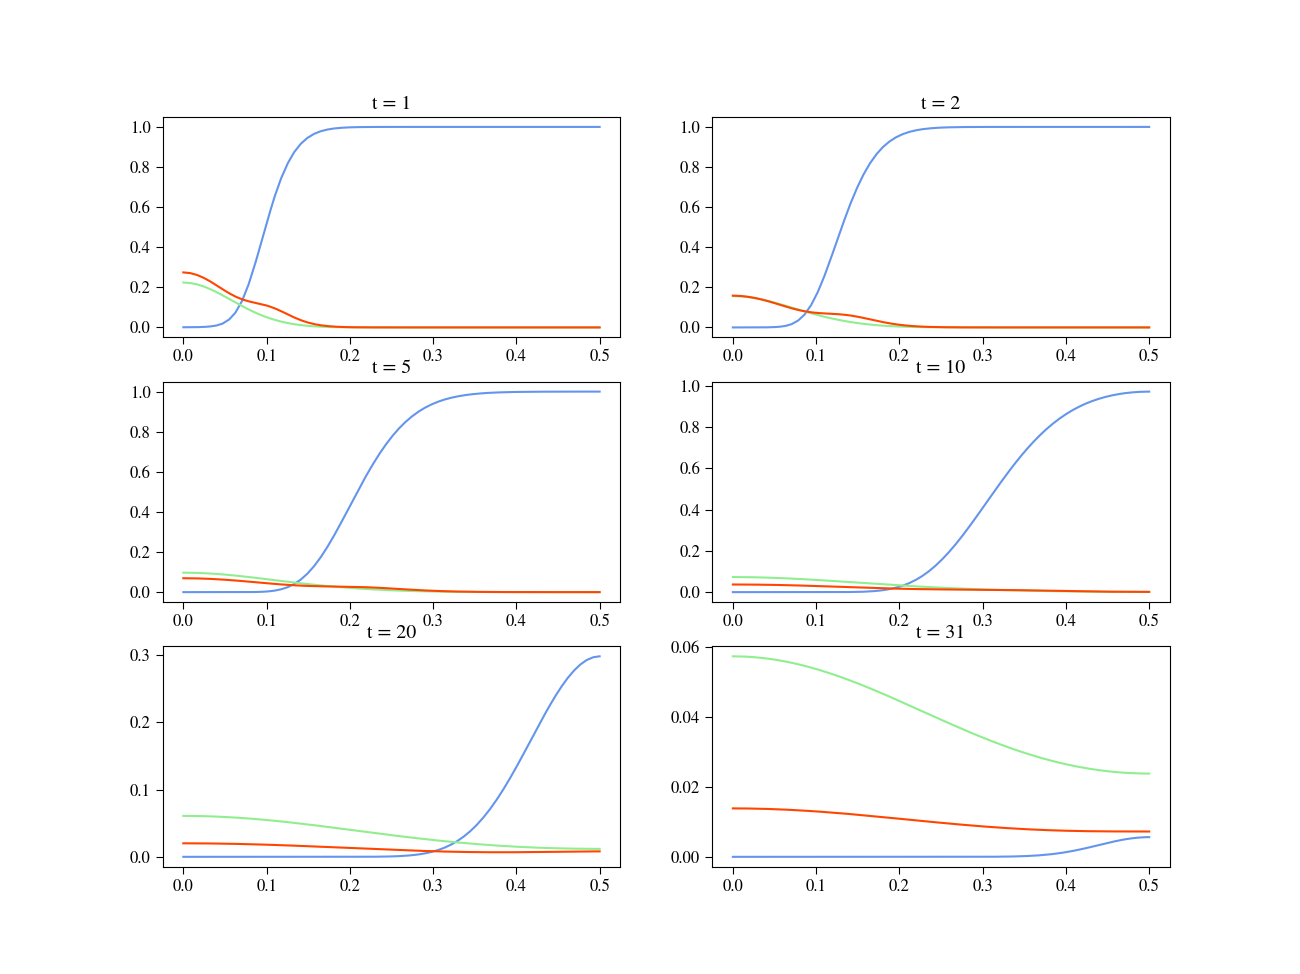
\includegraphics[width=\textwidth]{resources/images/0.001_0.001_0.001_20_0.1_0_0.002_0_0.png}
    \caption{Caption}
    \label{fig:0.001_0.001_0.001_20_0.1_0_0.002_0_0}
\end{figure}
In this last replicated experiment, shown by figure \ref{fig:0.001_0.001_0.001_20_0.1_0_0.002_0_0} the ECM degrading rate is increase with $\eta = 20$ and the haptotactic flux coefficient is decreased to a value of $\gamma = 0.002$. The adjustment of the haptotactic coefficient is noticable, the cluster forming at the leading edge of the tumour cells being as striking like in the first experiment. Where in the first experiment the value of the tumour density between the cluster and the origin, was visibly lower than the cluster itself, we can see no such behaviour here. The bump is distinguishable but in direction of the origin the curve does not flatten, on the contrary it is about 1.5 times hihger than the cluster itself. It is interesting to see, that although the degradation rate of the ECM is higher, form a temporaily point of view, the actual degradation does not happen faster than in experiment 1, this is due to the fact, the the haptotactic flux coefficient is decreased, the tumour cells don't migrate as fast into the surrouding tissue and therefore do not get as fast into contact with the ECM as in experiment 1. This interplay makes the ECM curve look over time like the one from experiment 1, althought the parameters for the experiments are noticably different. The MDE concentration looks like in experiment 1, though at the first pionts in time of the snapshots the concentration is higher towards the origin, since in this area are also more tumour cells producing it. \newline 
In all of the experiments except where decay and production rate of the MDE seemed to be in balance you can see that over time the MDE fulfill their task, degrading the ECM, which in some in point in time sooner or later results in higher values for the MDE than the ECM everywhere. 
\subsubsection{2D Parameter Analysis}
\subsection{3D Parameter Analysis}
\subsection{3D Simulations with heterogenous ECM structure}